\clearpage
\subsubsectionold{MSVC + \olly}
\myindex{\olly}

Загрузим пример в \olly и увидим, какие значения были установлены в EAX/EBX/ECX/EDX после исполнения CPUID: 

\begin{figure}[H]
\centering
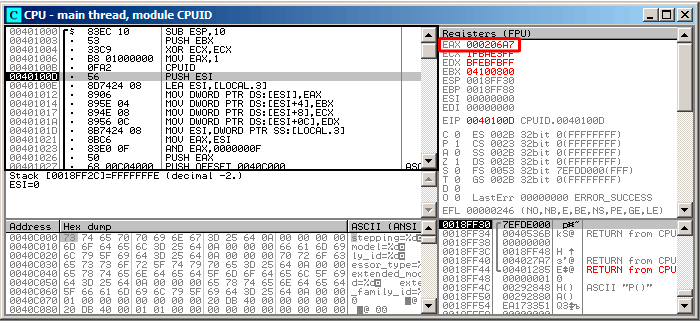
\includegraphics[scale=\FigScale]{patterns/15_structs/6_bitfields/cpuid/olly.png}
\caption{\olly: После исполнения CPUID}
\label{fig:cpuid_olly_1}
\end{figure}

В EAX установлено \TT{0x000206A7} (мой \ac{CPU} --- Intel Xeon E3-1220).\\
В двоичном виде это $0000 0000 0000 0010 0000 0110 1010 0111$.

Вот как распределяются биты по полям в моем случае:

\begin{center}
\begin{tabular}{ | l | l | l | }
\hline
\headercolor{} поле &
\headercolor{} в двоичном виде &
\headercolor{} в десятичном виде \\
\hline
reserved2		& 0000 & 0 \\
\hline
extended\_family\_id	& 00000000 & 0 \\
\hline
extended\_model\_id	& 0010 & 2 \\
\hline
reserved1		& 00 & 0 \\
\hline
processor\_id		& 00 & 0 \\
\hline
family\_id		& 0110 & 6 \\
\hline
model			& 1010 & 10 \\
\hline
stepping		& 0111 & 7 \\
\hline
\end{tabular}
\end{center}

\begin{figure}[H]
\centering
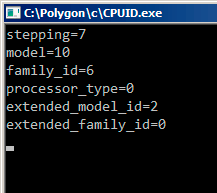
\includegraphics[scale=\NormalScale]{patterns/15_structs/6_bitfields/cpuid/result.png}
\caption{\olly: Результат работы}
\label{fig:cpuid_olly_2}
\end{figure}
